%% ============================================================
%%  FYP Presentation Slides — Project 16
%%  Optimizing Portering Logistics at HHH
%%  12-min presentation + 3-min video slot + 5-min Q&A
%% ============================================================
\documentclass[aspectratio=169,14pt]{beamer}

\usetheme{Madrid}
\usecolortheme{seahorse}
\setbeamertemplate{navigation symbols}{}
\setbeamertemplate{footline}[frame number]
\setbeamerfont{frametitle}{size=\large,series=\bfseries}

\usepackage[T1]{fontenc}
\usepackage[utf8]{inputenc}
\usepackage{lmodern}
\usepackage{CJKutf8}
\usepackage{booktabs}
\usepackage{array}
\usepackage{amsmath}
\usepackage{xcolor}
\usepackage{tikz}
\usetikzlibrary{shapes.geometric, arrows.meta, positioning, backgrounds}
\usepackage{pgfplots}
\pgfplotsset{compat=1.18}

%% Custom colours
\definecolor{hkustblue}{RGB}{0,51,102}
\definecolor{hkustgold}{RGB}{192,148,59}
\definecolor{alertred}{RGB}{180,30,30}
\definecolor{okgreen}{RGB}{30,130,60}

\setbeamercolor{frametitle}{bg=hkustblue,fg=white}
\setbeamercolor{title}{bg=hkustblue,fg=white}
\setbeamercolor{structure}{fg=hkustblue}
\setbeamercolor{alerted text}{fg=alertred}

%% Helpers
\newcommand{\tick}{\textcolor{okgreen}{\textbf{\checkmark}}}
\newcommand{\cross}{\textcolor{alertred}{\textbf{\texttimes}}}
\newcommand{\highlight}[1]{\colorbox{hkustgold!30}{\textbf{#1}}}

% ============================================================
\begin{document}
% ============================================================

%% ---- TITLE SLIDE ----
\begin{frame}
\vspace{0.5cm}
\begin{center}
  {\color{hkustblue}\rule{\linewidth}{2pt}}\\[0.4cm]
  {\Large\bfseries\color{hkustblue} Optimizing Portering Logistics at HHH}\\[0.2cm]
  {\large An AI-Driven Porter Dispatch System}\\[0.4cm]
  {\color{hkustblue}\rule{\linewidth}{2pt}}\\[0.6cm]

  \begin{columns}[t]
    \column{0.5\textwidth}
    \centering
    {\small\textbf{Team Members}}\\[0.2cm]
    {\small CHAN Hok Nam\\CHOI Cheuk Man\\KIM Youseung}
    \column{0.5\textwidth}
    \centering
    {\small\textbf{Supervisor}}\\[0.2cm]
    {\small Prof.\ Xiangtong QI}\\[0.3cm]
    {\small Project 16 $\cdot$ IEDA FYP 2025--26}
  \end{columns}

  \vspace{0.5cm}
  {\footnotesize Department of Industrial Engineering \& Decision Analytics, HKUST}
\end{center}
\end{frame}

%% ---- AGENDA ----
\begin{frame}{Presentation Outline}
\begin{columns}
\column{0.55\textwidth}
\begin{enumerate}
  \setlength{\itemsep}{8pt}
  \item \textbf{The Problem} — Why does this matter?
  \item \textbf{Our Solution} — System architecture
  \item \textbf{How accurate is the AI parsing?}
  \item \textbf{Does the optimizer actually help?}
  \item \textbf{Live demo highlights}
  \item \textbf{Conclusion \& Future work}
\end{enumerate}

\column{0.4\textwidth}
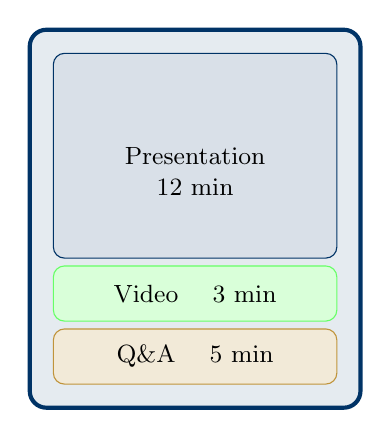
\begin{tikzpicture}
  \draw[fill=hkustblue!10, draw=hkustblue, rounded corners=6pt, line width=1.5pt]
    (0,0) rectangle (4.2,4.8);
  \node[font=\small\bfseries, color=hkustblue] at (2.1,4.3) {12-min talk};
  \draw[fill=hkustgold!20, draw=hkustgold, rounded corners=4pt]
    (0.3,0.3) rectangle (3.9,1.0);
  \node[font=\small] at (2.1,0.65) {Q\&A \quad 5 min};
  \draw[fill=green!15, draw=green!60, rounded corners=4pt]
    (0.3,1.1) rectangle (3.9,1.8);
  \node[font=\small] at (2.1,1.45) {Video \quad 3 min};
  \draw[fill=hkustblue!15, draw=hkustblue, rounded corners=4pt]
    (0.3,1.9) rectangle (3.9,4.5);
  \node[font=\small] at (2.1,3.2) {Presentation};
  \node[font=\small] at (2.1,2.8) {12 min};
\end{tikzpicture}
\end{columns}
\end{frame}

%% ==============================================================
%% SECTION 1 — THE PROBLEM
%% ==============================================================

\begin{frame}{The Problem: Porter Dispatch at HHH}
\begin{columns}
\column{0.48\textwidth}
\textbf{What porters do:}
\begin{itemize}
  \item Transport patients, specimens, equipment between departments
  \item Operate 24/7 across entire hospital
  \item Dispatched manually by radio
\end{itemize}

\vspace{0.4cm}
\textbf{HHH's stated KPI:}
\begin{center}
  \fbox{\Large\bfseries Every task $\leq$ 15 minutes}
\end{center}

\column{0.48\textwidth}
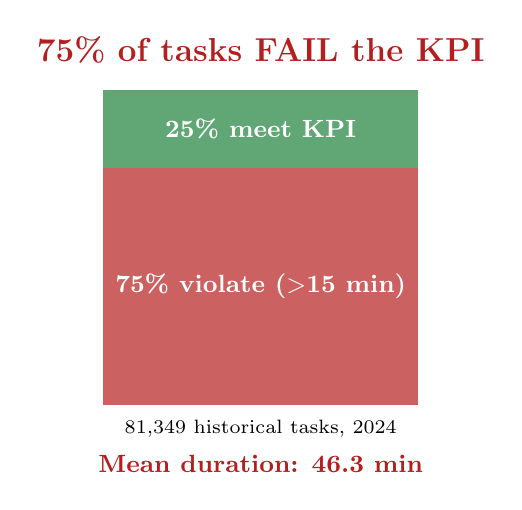
\begin{tikzpicture}
  %% Simple bar showing violation
  \node[font=\bfseries\large, color=alertred] at (2.5, 4.5)
    {75\% of tasks FAIL the KPI};

  %% Stacked bar
  \fill[alertred!70] (0.5,0) rectangle (4.5,3.0);
  \fill[okgreen!70]  (0.5,3.0) rectangle (4.5,4.0);
  \node[font=\small\bfseries, color=white] at (2.5,1.5) {75\% violate ($>$15 min)};
  \node[font=\small\bfseries, color=white] at (2.5,3.5) {25\% meet KPI};

  %% Labels
  \node[font=\scriptsize] at (2.5,-0.3) {81,349 historical tasks, 2024};
  \node[font=\small\bfseries, color=alertred] at (2.5,-0.75)
    {Mean duration: \textbf{46.3 min}};
\end{tikzpicture}
\end{columns}
\end{frame}

\begin{frame}{Root Causes of Poor KPI Performance}
\begin{columns}
\column{0.52\textwidth}

\textbf{By service type (pickup violation rate):}

\vspace{0.2cm}
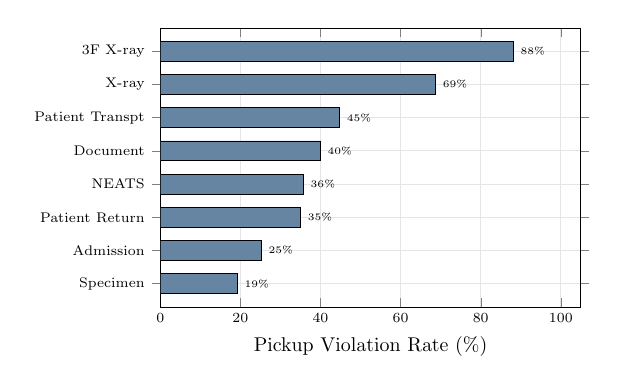
\begin{tikzpicture}[scale=0.72]
\begin{axis}[
  xbar,
  bar width=10pt,
  width=9cm, height=6.5cm,
  xlabel={Pickup Violation Rate (\%)},
  xmin=0, xmax=105,
  symbolic y coords={
    {Specimen},{Admission},{Patient Return},{NEATS},{Document},{Patient Transpt},{X-ray},{3F X-ray}},
  ytick=data,
  y tick label style={font=\scriptsize},
  x tick label style={font=\scriptsize},
  nodes near coords={\pgfmathprintnumber[precision=0]{\pgfplotspointmeta}\%},
  nodes near coords style={font=\tiny},
  grid=major, grid style={gray!20},
]
\addplot[fill=hkustblue!60] coordinates {
  (19.3,{Specimen})
  (25.3,{Admission})
  (35.1,{Patient Return})
  (35.8,{NEATS})
  (40.0,{Document})
  (44.8,{Patient Transpt})
  (68.8,{X-ray})
  (88.2,{3F X-ray})
};
\end{axis}
\end{tikzpicture}

\column{0.44\textwidth}
\vspace{-0.5cm}
\begin{block}{Key insight}
  3F X-ray has the highest pickup violation rate (88.2\%) --- imaging suites concentrate on specific floors, leaving few porters geographically near the pickup origin.
\end{block}

\vspace{0.3cm}
\textbf{Three dispatch problems:}
\begin{enumerate}
  \item[\cross] Manual, radio-based assignment
  \item[\cross] No global fleet optimisation
  \item[\cross] No structured data capture
\end{enumerate}
\end{columns}
\end{frame}

%% ==============================================================
%% SECTION 2 — SOLUTION
%% ==============================================================

\begin{frame}{Our Solution: Hybrid AI Dispatch System}
\begin{center}
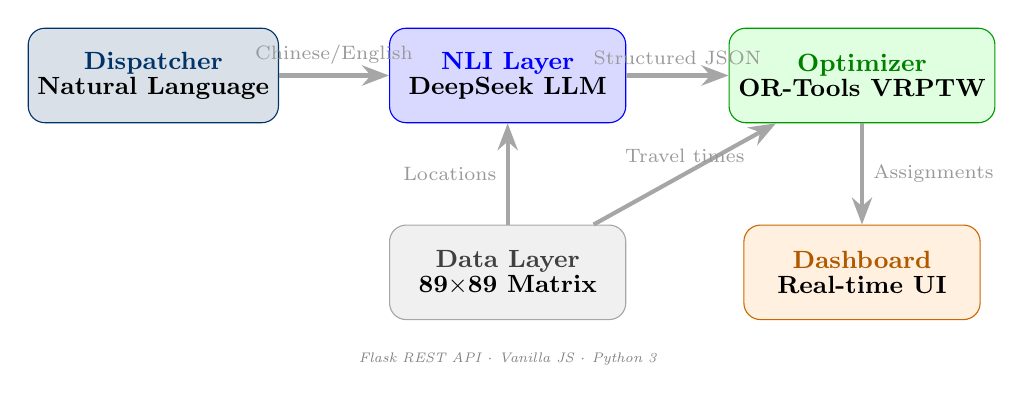
\begin{tikzpicture}[
  arr/.style={-Stealth, thick, gray!70, line width=1.5pt},
  lbl/.style={font=\scriptsize, color=gray!80},
  nodebox/.style={rectangle, rounded corners=6pt, minimum width=3.0cm, minimum height=1.2cm, align=center, font=\small\bfseries}
]

\node[nodebox, draw=hkustblue, fill=hkustblue!15] (in)   at (-4.5, 0) {\color{hkustblue}Dispatcher\\[-2pt]Natural Language};
\node[nodebox, draw=blue, fill=blue!15]            (nlp)  at (0, 0)   {\color{blue}NLI Layer\\[-2pt]DeepSeek LLM};
\node[nodebox, draw=green!60!black, fill=green!12] (vrp)  at (4.5, 0) {\color{green!50!black}Optimizer\\[-2pt]OR-Tools VRPTW};
\node[nodebox, draw=orange!80!black, fill=orange!12](ui)  at (4.5,-2.5){\color{orange!70!black}Dashboard\\[-2pt]Real-time UI};
\node[nodebox, draw=gray!70, fill=gray!12]         (data) at (0, -2.5) {\color{gray!50!black}Data Layer\\[-2pt]89$\times$89 Matrix};

\draw[arr] (in) -- node[above,lbl]{Chinese/English} (nlp);
\draw[arr] (nlp) -- node[above,lbl]{Structured JSON} (vrp);
\draw[arr] (vrp) -- node[right,lbl]{Assignments} (ui);
\draw[arr] (data) -- node[above,lbl]{Travel times} (vrp);
\draw[arr] (data) -- node[left,lbl]{Locations} (nlp);

\node[font=\tiny\itshape, color=gray] at (0, -3.6) {Flask REST API $\cdot$ Vanilla JS $\cdot$ Python 3};
\end{tikzpicture}
\end{center}
\end{frame}

\begin{frame}{What the System Does — End to End}
\begin{columns}
\column{0.47\textwidth}

\textbf{Step 1 — Dispatcher types:}
\begin{exampleblock}{}
  \small``Super urgent patient from A\&D to SDU''
\end{exampleblock}

\vspace{0.3cm}
\textbf{Step 2 — LLM parses:}
\begin{exampleblock}{}
  \small\texttt{\{from: "A\&D", to: "SDU",}\\
  \texttt{ service: "admission",}\\
  \texttt{ priority: "Super-Urgent"\}}
\end{exampleblock}

\vspace{0.3cm}
\textbf{Step 3 — Solver assigns:}
\begin{exampleblock}{}
  \small Porter P-003 (nearest, 1.2 min away)\\
  Estimated total: \textbf{8.4 min}
\end{exampleblock}

\column{0.50\textwidth}
\textbf{Features at a glance:}
\begin{itemize}
  \setlength{\itemsep}{5pt}
  \item[\tick] Chinese \& English NL input
  \item[\tick] Multi-task from one request
  \item[\tick] Intermediate stops / waypoints
  \item[\tick] Infection control flags (VRE, NEATS)
  \item[\tick] Scheduled future tasks
  \item[\tick] Rolling-horizon re-optimisation
  \item[\tick] LLM ``Why this porter?'' explanation
  \item[\tick] RAG policy advisor
  \item[\tick] Undo last dispatch
\end{itemize}
\end{columns}
\end{frame}

%% ==============================================================
%% SECTION 3 — NLP ACCURACY (anticipated Q&A question)
%% ==============================================================

\begin{frame}{How Accurate Is the LLM Parsing? \hfill\small\color{hkustgold}[Tested on 100 samples]}

\begin{columns}
\column{0.50\textwidth}

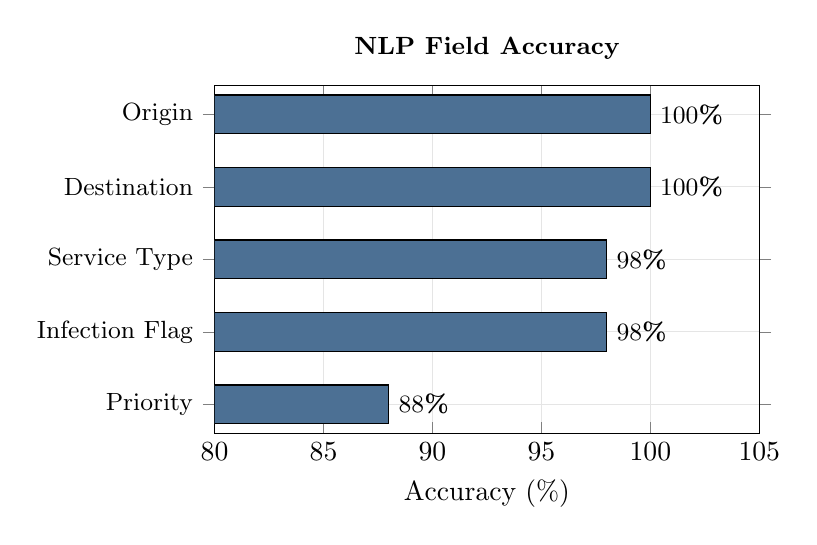
\begin{tikzpicture}
\begin{axis}[
  xbar,
  bar width=14pt,
  width=8.5cm, height=6cm,
  xlabel={Accuracy (\%)},
  xmin=80, xmax=105,
  symbolic y coords={Priority,Infection Flag,Service Type,Destination,Origin},
  ytick=data,
  y tick label style={font=\small},
  nodes near coords={\pgfmathprintnumber[precision=1]{\pgfplotspointmeta}\%},
  nodes near coords style={font=\small\bfseries},
  grid=major, grid style={gray!20},
  title={NLP Field Accuracy},
  title style={font=\small\bfseries},
]
\addplot[fill=hkustblue!70] coordinates {
  (88.0,Priority)
  (98.0,{Infection Flag})
  (98.0,{Service Type})
  (100.0,Destination)
  (100.0,Origin)
};
\end{axis}
\end{tikzpicture}

\column{0.46\textwidth}
\vspace{-0.3cm}

\begin{alertblock}{84\% all-5-fields correct}
Zero LLM parse failures across 100 samples.
\end{alertblock}

\vspace{0.3cm}
\textbf{Priority: 88\%}\\
{\small All 12 errors: ``Immediate'' (\begin{CJK}{UTF8}{min}即時\end{CJK}) parsed as Normal instead of Urgent. Systematic, fixable with one prompt rule.}

\vspace{0.3cm}
\textbf{Location: 100\%}\\
{\small Achieved because all 89 locations are enumerated in the system prompt.}

\vspace{0.3cm}
\begin{exampleblock}{Verdict}
  Reliable for production dispatch.\\
  Priority rule fix would push to $\sim$96\%.
\end{exampleblock}

\end{columns}
\end{frame}

%% ==============================================================
%% SECTION 4 — DOES THE OPTIMIZER HELP?
%% ==============================================================

\begin{frame}{Does the Optimizer Actually Help?}
\begin{columns}
\column{0.54\textwidth}

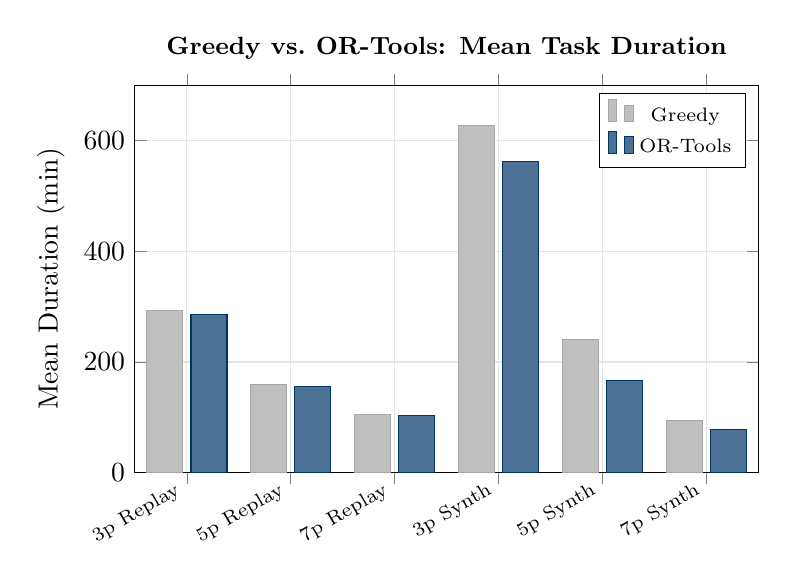
\begin{tikzpicture}
\begin{axis}[
  ybar=3pt,
  bar width=13pt,
  width=9.5cm, height=6.5cm,
  symbolic x coords={3p Replay,5p Replay,7p Replay,3p Synth,5p Synth,7p Synth},
  xtick=data,
  x tick label style={rotate=30, anchor=east, font=\scriptsize},
  ylabel={Mean Duration (min)},
  ymin=0, ymax=700,
  legend style={at={(0.98,0.98)}, anchor=north east, font=\scriptsize},
  grid=major, grid style={gray!20},
  title={Greedy vs.\ OR-Tools: Mean Task Duration},
  title style={font=\small\bfseries},
]
\addplot[fill=gray!50, draw=gray!70] coordinates {
  (3p Replay, 293.5)(5p Replay, 158.6)(7p Replay, 104.4)
  (3p Synth, 627.4)(5p Synth, 240.0)(7p Synth, 94.1)
};
\addplot[fill=hkustblue!70, draw=hkustblue] coordinates {
  (3p Replay, 286.6)(5p Replay, 155.1)(7p Replay, 103.4)
  (3p Synth, 563.2)(5p Synth, 166.8)(7p Synth, 78.2)
};
\legend{Greedy, OR-Tools}
\end{axis}
\end{tikzpicture}

\column{0.43\textwidth}
\vspace{-0.3cm}

\begin{block}{Key finding}
  OR-Tools helps most when the system is \textbf{not saturated}.
\end{block}

\vspace{0.3cm}
\textbf{Under light load (synthetic):}
\begin{itemize}
  \item 5 porters: \highlight{30.5\% improvement}
  \item 7 porters: \highlight{16.9\% improvement}
\end{itemize}

\vspace{0.3cm}
\textbf{Under real HHH load (replay):}
\begin{itemize}
  \item Marginal gains (0.5--2\%)
  \item System is queue-saturated
  \item Routing can't overcome fleet shortage
\end{itemize}

\end{columns}
\end{frame}

\begin{frame}{What Does the 15-min KPI Actually Mean?}
\begin{columns}
\column{0.52\textwidth}

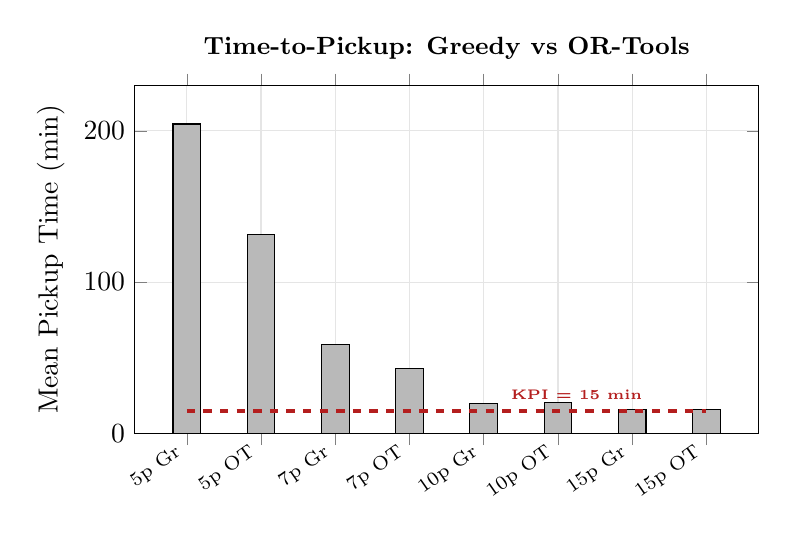
\begin{tikzpicture}
\begin{axis}[
  ybar=2pt,
  bar width=10pt,
  width=9.5cm, height=6.0cm,
  symbolic x coords={5p Gr,5p OT,7p Gr,7p OT,10p Gr,10p OT,15p Gr,15p OT},
  xtick=data,
  x tick label style={rotate=35, anchor=east, font=\scriptsize},
  ylabel={Mean Pickup Time (min)},
  ymin=0, ymax=230,
  grid=major, grid style={gray!20},
  title={Time-to-Pickup: Greedy vs OR-Tools},
  title style={font=\small\bfseries},
  legend style={at={(0.98,0.98)}, anchor=north east, font=\tiny},
]
\addplot[fill=gray!55] coordinates {
  (5p Gr,204.5)(5p OT,131.3)(7p Gr,58.6)(7p OT,42.7)
  (10p Gr,20.0)(10p OT,20.1)(15p Gr,15.9)(15p OT,15.9)
};
\draw[dashed, alertred, line width=1.5pt]
  (axis cs:5p Gr,15) -- (axis cs:15p OT,15)
  node[pos=0.75, above, font=\tiny\bfseries, color=alertred]{KPI = 15 min};
\end{axis}
\end{tikzpicture}

\column{0.45\textwidth}
\vspace{-0.3cm}

\begin{block}{KPI definition}
  15 min = porter \textbf{arrives at pickup}\\
  (response time), not task completion.
\end{block}

\vspace{0.2cm}
\textbf{OR-Tools pickup improvement:}
\begin{itemize}
  \item 5 porters: \highlight{35.8\% faster}
  \item 7 porters: \highlight{27.2\% faster}
\end{itemize}

\vspace{0.2cm}
\begin{exampleblock}{Fleet-sizing finding}
  \textbf{15 porters + OR-Tools:}\\
  Mean pickup = \textbf{15.9 min} $\approx$ KPI
\end{exampleblock}

\vspace{0.2cm}
{\scriptsize\color{gray} 57.0\% of routes: full task $>$15 min regardless of algorithm (fixed by geography, not dispatch)}

\end{columns}
\end{frame}

%% ==============================================================
%% SECTION 5 — DEMO HIGHLIGHTS
%% ==============================================================

\begin{frame}{System Demo Highlights}
\begin{columns}
\column{0.48\textwidth}

\textbf{Real-time Dashboard}

\vspace{0.2cm}
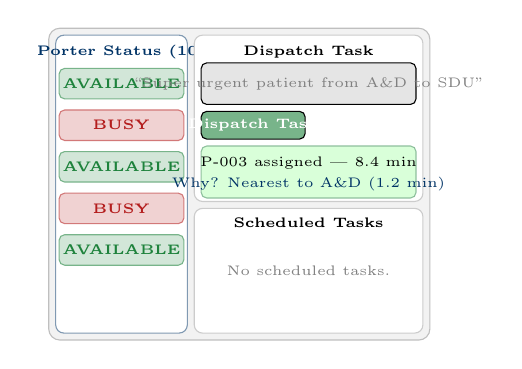
\begin{tikzpicture}[scale=0.88]
  %% Mock dashboard layout
  \draw[fill=gray!10, draw=gray!50, rounded corners=4pt] (0,0) rectangle (5.5,4.5);

  %% Porter status panel
  \draw[fill=white, draw=hkustblue!50, rounded corners=3pt] (0.1,0.1) rectangle (2.0,4.4);
  \node[font=\tiny\bfseries, color=hkustblue] at (1.05,4.15) {Porter Status (10)};
  \foreach \y/\col/\st in {3.7/okgreen/AVAILABLE, 3.1/alertred/BUSY, 2.5/okgreen/AVAILABLE,
                            1.9/alertred/BUSY, 1.3/okgreen/AVAILABLE}{
    \draw[fill=\col!20, draw=\col!60, rounded corners=2pt] (0.15,\y-0.22) rectangle (1.95,\y+0.22);
    \node[font=\tiny, color=\col] at (1.05,\y) {\textbf{\st}};
  }

  %% Dispatch panel
  \draw[fill=white, draw=gray!40, rounded corners=3pt] (2.1,2.0) rectangle (5.4,4.4);
  \node[font=\tiny\bfseries] at (3.75,4.15) {Dispatch Task};
  \draw[fill=gray!20, rounded corners=2pt] (2.2,3.4) rectangle (5.3,4.0);
  \node[font=\tiny, color=gray] at (3.75,3.7) {``Super urgent patient from A\&D to SDU''};
  \draw[fill=okgreen!60, rounded corners=2pt] (2.2,2.9) rectangle (3.7,3.3);
  \node[font=\tiny\bfseries, color=white] at (2.95,3.1) {Dispatch Task};
  \draw[fill=green!15, draw=okgreen!50, rounded corners=2pt] (2.2,2.05) rectangle (5.3,2.8);
  \node[font=\tiny] at (3.75,2.55) {P-003 assigned | 8.4 min};
  \node[font=\tiny, color=hkustblue] at (3.75,2.25) {Why? Nearest to A\&D (1.2 min)};

  %% Queue indicator
  \draw[fill=white, draw=gray!40, rounded corners=3pt] (2.1,0.1) rectangle (5.4,1.9);
  \node[font=\tiny\bfseries] at (3.75,1.7) {Scheduled Tasks};
  \node[font=\tiny, color=gray] at (3.75,1.0) {No scheduled tasks.};
\end{tikzpicture}

\column{0.48\textwidth}

\textbf{Policy Advisor (RAG)}

\vspace{0.2cm}
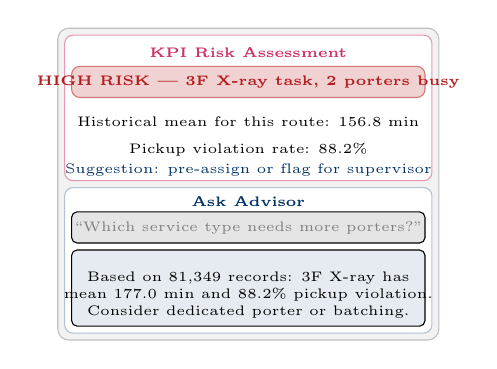
\begin{tikzpicture}[scale=0.88]
  \draw[fill=gray!10, draw=gray!50, rounded corners=4pt] (0,0) rectangle (5.5,4.5);

  %% Risk assessment
  \draw[fill=white, draw=purple!40, rounded corners=3pt] (0.1,2.3) rectangle (5.4,4.4);
  \node[font=\tiny\bfseries, color=purple!80] at (2.75,4.15) {KPI Risk Assessment};
  \draw[fill=alertred!20, draw=alertred!60, rounded corners=3pt] (0.2,3.5) rectangle (5.3,3.95);
  \node[font=\tiny\bfseries, color=alertred] at (2.75,3.72) {HIGH RISK — 3F X-ray task, 2 porters busy};
  \node[font=\tiny] at (2.75,3.15) {Historical mean for this route: 156.8 min};
  \node[font=\tiny] at (2.75,2.75) {Pickup violation rate: 88.2\%};
  \node[font=\tiny, color=hkustblue] at (2.75,2.45) {Suggestion: pre-assign or flag for supervisor};

  %% Q&A
  \draw[fill=white, draw=hkustblue!30, rounded corners=3pt] (0.1,0.1) rectangle (5.4,2.2);
  \node[font=\tiny\bfseries, color=hkustblue] at (2.75,2.0) {Ask Advisor};
  \draw[fill=gray!20, rounded corners=2pt] (0.2,1.4) rectangle (5.3,1.85);
  \node[font=\tiny, color=gray] at (2.75,1.62) {``Which service type needs more porters?''};
  \draw[fill=hkustblue!10, rounded corners=2pt] (0.2,0.2) rectangle (5.3,1.3);
  \node[font=\tiny] at (2.75,0.9) {Based on 81,349 records: 3F X-ray has};
  \node[font=\tiny] at (2.75,0.65) {mean 177.0 min and 88.2\% pickup violation.};
  \node[font=\tiny] at (2.75,0.4) {Consider dedicated porter or batching.};
\end{tikzpicture}

\end{columns}
\end{frame}

%% ==============================================================
%% SECTION 6 — CONCLUSION
%% ==============================================================

\begin{frame}{Summary of Contributions}
\begin{columns}
\column{0.55\textwidth}

\begin{block}{1. Validated NLI (LLM layer)}
  \begin{itemize}
    \item 84\% all-field accuracy on 100 real samples
    \item 100\% location extraction
    \item Handles Chinese, multi-task, constraints
  \end{itemize}
\end{block}

\vspace{0.3cm}
\begin{block}{2. OR-Tools VRPTW Solver}
  \begin{itemize}
    \item Pickup time: up to \textbf{35.8\%} faster than greedy
    \item Total duration: up to \textbf{30.5\%} improvement
    \item 15 porters $\Rightarrow$ mean pickup $\approx$ KPI target
  \end{itemize}
\end{block}

\vspace{0.3cm}
\begin{block}{3. Operational Intelligence}
  \begin{itemize}
    \item RAG policy advisor over 81,349 historical tasks
    \item KPI risk, fleet recommendations, free-text Q\&A
  \end{itemize}
\end{block}

\column{0.42\textwidth}

\textbf{Deliverables:}
\begin{itemize}
  \setlength{\itemsep}{5pt}
  \item[\tick] Deployed web app (Flask)
  \item[\tick] 89$\times$89 travel matrix
  \item[\tick] Discrete-event simulator
  \item[\tick] NLP accuracy test harness
  \item[\tick] Policy advisor (RAG)
  \item[\tick] Simulation benchmarks
\end{itemize}

\vspace{0.5cm}
\textbf{Future work:}
\begin{itemize}
  \item SQLite persistent storage
  \item Infection control routing
  \item Real-time location integration
  \item HHH field trial
\end{itemize}

\end{columns}
\end{frame}

%% ---- FINAL SLIDE ----
\begin{frame}
\begin{center}
  \vspace{1cm}
  {\color{hkustblue}\rule{\linewidth}{2pt}}\\[0.8cm]
  {\Huge\bfseries\color{hkustblue} Thank You}\\[0.6cm]
  {\Large Questions Welcome}\\[0.8cm]
  {\color{hkustblue}\rule{\linewidth}{2pt}}

  \vspace{0.8cm}
  \begin{columns}
    \column{0.33\textwidth}\centering
    {\small CHAN Hok Nam}
    \column{0.33\textwidth}\centering
    {\small CHOI Cheuk Man}
    \column{0.33\textwidth}\centering
    {\small KIM Youseung}
  \end{columns}

  \vspace{0.4cm}
  {\footnotesize Supervisor: Prof.\ Xiangtong QI $\cdot$ Project 16 $\cdot$ IEDA HKUST 2025--26}
\end{center}
\end{frame}

%% ==============================================================
%% BACKUP SLIDES (for Q&A)
%% ==============================================================

\begin{frame}[plain]
\begin{center}
  \vspace{1.5cm}
  {\Large\bfseries\color{gray} BACKUP SLIDES}\\[0.2cm]
  {\small for Q\&A reference}
\end{center}
\end{frame}

\begin{frame}{Backup: OR-Tools Formulation Details}
\begin{columns}
\column{0.5\textwidth}
\textbf{Node graph:}
\begin{itemize}
  \item $m$ porter start depots
  \item $n$ pickup nodes (task origins)
  \item $n$ delivery nodes (task destinations)
  \item 1 dummy end depot
\end{itemize}

\textbf{Objective:}
\[
\min \sum_{(i,j)} c_{ij} + \lambda \sum_k \max(0, \text{done}_k - 15)
\]
$\lambda = 1000$ centi-min per minute over KPI

\column{0.5\textwidth}
\textbf{Constraints:}
\begin{itemize}
  \item Pickup before delivery (same porter)
  \item Capacity: 1 task at a time per porter
  \item Drop penalty $2\times10^7 \gg$ any KPI penalty
  \item 1-second solve limit
\end{itemize}

\textbf{Search strategy:}\\
PARALLEL\_CHEAPEST\_INSERTION\\
$\Rightarrow$ GUIDED\_LOCAL\_SEARCH

\textbf{Fallback:} Greedy (nearest available)
\end{columns}
\end{frame}

\begin{frame}{Backup: Why Not Train a Custom NLP Model?}
\begin{columns}
\column{0.5\textwidth}
\textbf{Option A: Trained classifier}
\begin{itemize}
  \item[\cross] Requires labelled training data
  \item[\cross] 84,000 records need annotation
  \item[\cross] Domain shift if terminology changes
  \item[\tick] Higher ceiling accuracy
\end{itemize}

\vspace{0.4cm}
\textbf{Option B: LLM with prompt (chosen)}
\begin{itemize}
  \item[\tick] No annotation required
  \item[\tick] Handles unseen phrasings
  \item[\tick] Easy to update (change prompt)
  \item[\cross] API cost per request
  \item[\cross] 88\% priority accuracy
\end{itemize}

\column{0.5\textwidth}
\begin{exampleblock}{Practical verdict}
  For a hospital prototype without labelled data, the LLM approach is the right engineering choice. 84\% all-field accuracy is sufficient for dispatch with human oversight.\\[0.3cm]
  A trained model would be the natural next step if HHH commits to deployment and provides annotated records.
\end{exampleblock}
\end{columns}
\end{frame}

\begin{frame}{Backup: Pickup-Time KPI Analysis}
\centering
\footnotesize
\begin{tabular}{cccc}
\toprule
\textbf{Porters} & \textbf{Strategy} & \textbf{Mean Pickup (min)} & \textbf{Pickup Violation (\%)} \\
\midrule
5  & Greedy   & 204.5 & 96.0\% \\
5  & OR-Tools & \textbf{131.3} & \textbf{83.0\%} \\
7  & Greedy   & 58.6  & 94.0\% \\
7  & OR-Tools & \textbf{42.7}  & \textbf{78.0\%} \\
10 & Greedy   & 20.0  & 59.0\% \\
10 & OR-Tools & 20.1  & 60.0\% \\
15 & Either   & \textbf{15.9}  & \textbf{48.0\%} \\
\bottomrule
\end{tabular}

\vspace{0.4cm}
{\small Synthetic mode $\cdot$ 100 tasks $\cdot$ 8-min mean inter-arrival (historically realistic)}\\[0.2cm]
{\small 57.0\% of all routes have direct travel + service time $>$15 min --- KPI blocks are geographic for these tasks}
\end{frame}

\begin{frame}{Backup: Full Simulation Data}
\centering
\footnotesize
\begin{tabular}{llcc}
\toprule
\textbf{Mode} & \textbf{Strategy} & \textbf{Porters} & \textbf{Mean Total Duration (min)} \\
\midrule
Replay    & Greedy   & 3 & 293.5 \\
Replay    & OR-Tools & 3 & 286.6 \\
Replay    & Greedy   & 5 & 158.6 \\
Replay    & OR-Tools & 5 & 155.1 \\
Replay    & Greedy   & 7 & 104.4 \\
Replay    & OR-Tools & 7 & 103.4 \\
\midrule
Synthetic & Greedy   & 3 & 627.4 \\
Synthetic & OR-Tools & 3 & 563.2 \\
Synthetic & Greedy   & 5 & 240.0 \\
Synthetic & OR-Tools & 5 & 166.8 \\
Synthetic & Greedy   & 7 & 94.1  \\
Synthetic & OR-Tools & 7 & 78.2  \\
\bottomrule
\end{tabular}
\end{frame}

\end{document}
